\section{Design Brief and Method for the Dynamic Honeycomb Maze}



\subsection{Dynamic Honeycomb Maze Brief}
\label{section:design_brief}

\begin{figure}[h]
    \centering
    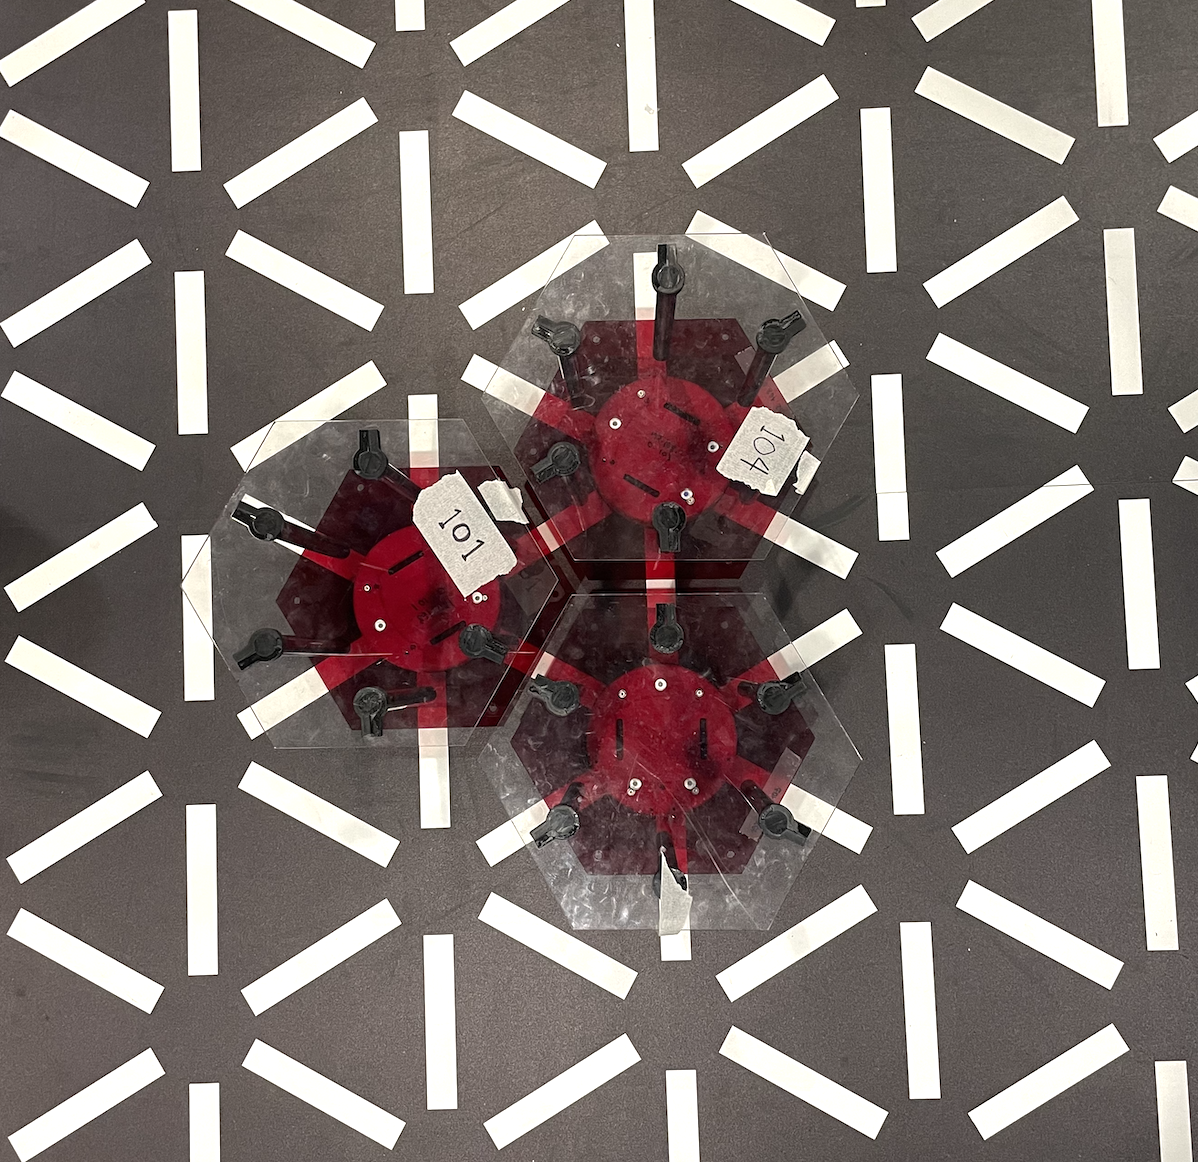
\includegraphics[scale=0.35]{images/irl_maze.png}
    \caption{This figure shows a top down view of one of the configurations of the honeycomb maze where there a hexagonal grid where the hexagonal robots are placed on top. Upon one of these platforms the animal would be placed on the hexagons and would choose which platform to move to.}
    \label{fig:picture_of_maze}
\end{figure}

There are three platforms on the hexagon space and one has the animal placed on it. They is all placed in a room with the hexagonal grid marking on the floor, representing the maze that the animal traverses.

The stated goal of the algorithm is as follows:
\begin{enumerate}
    \item(Fig. \ref{fig:example_algorithm} Panel A) The animal is placed on a platform robot with is consecutive to two other platforms. It can either chose to move to one platform or the other. This is entirely the mouse's decision (shown in Fig. \ref{fig:example_algorithm} panel B).
    \item After the mouse has made this choice, it must move the remaining platforms \textit{without} the animal on it so they are newly positioned next to the new platform with the animal on it (as shown in fig. \ref{fig:example_algorithm} panel C).
    \item This cycle will continue until the mouse has reach the goal required by the experimenter.
\end{enumerate}

An example of what the function of the algorithm's function is, is shown in Figure \ref{fig:example_algorithm}. Note that in this figure the arrangements of the hexagons around the central green platform are examples only. They can be placed anywhere around the central green platform as shown in panel C of Figure \ref{fig:example_algorithm}.

\begin{figure}[H]
    \centering
    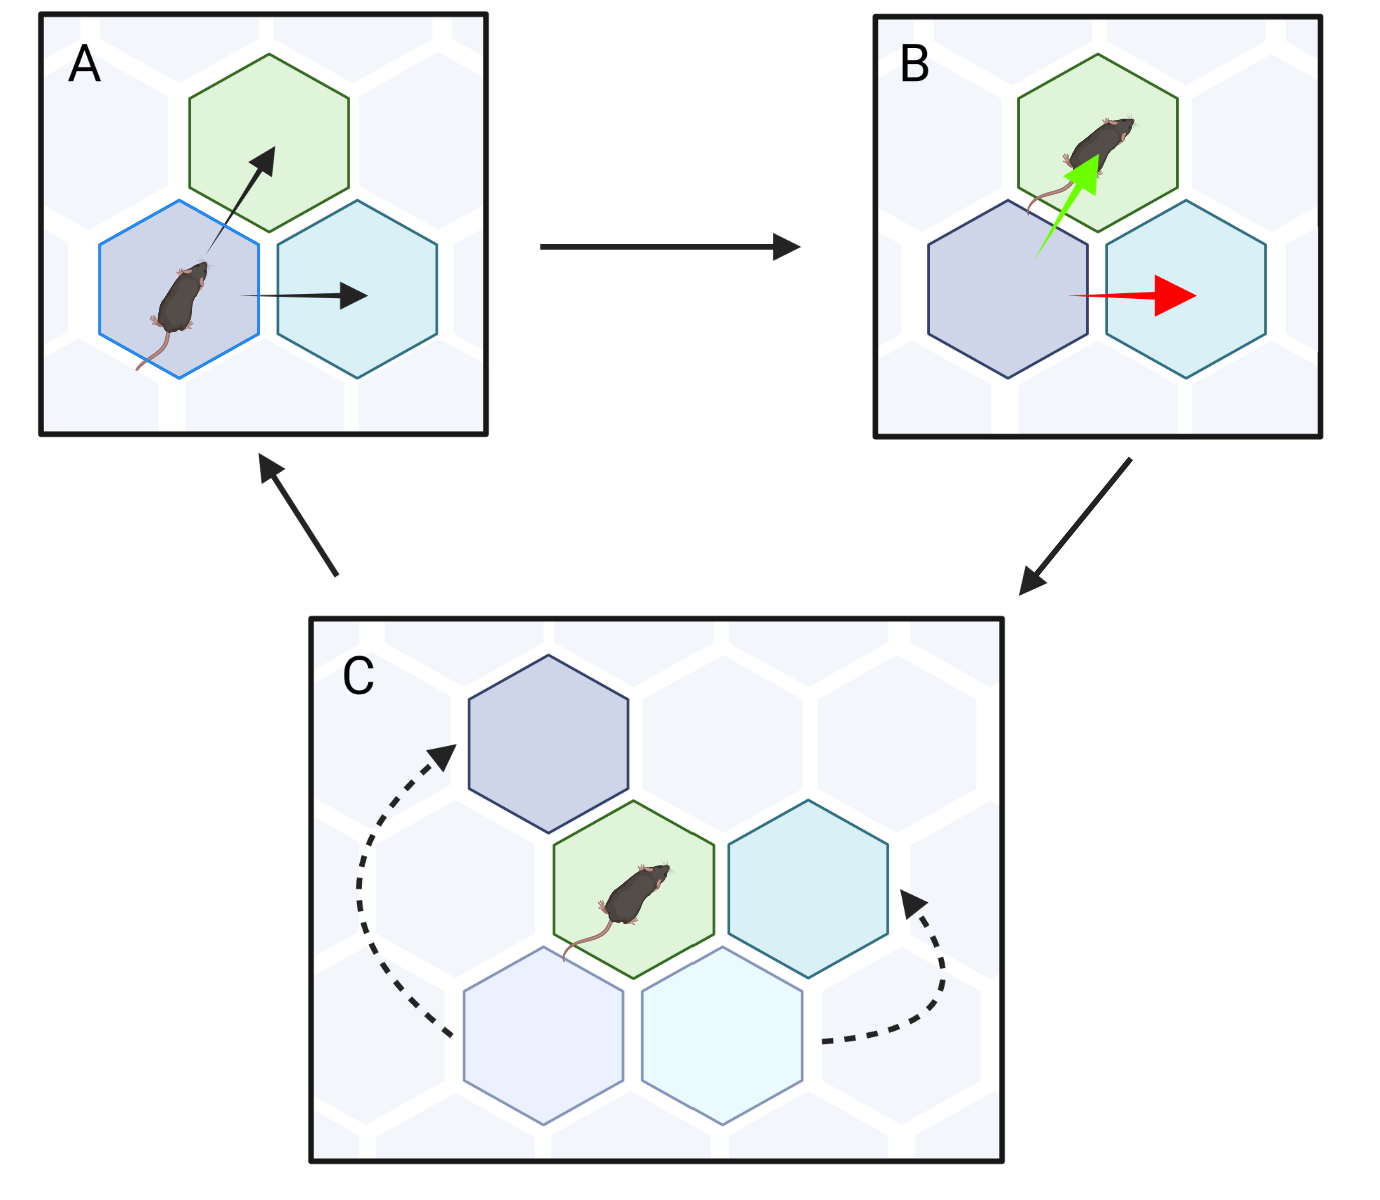
\includegraphics[scale=0.6]{images/example_algorithm.png}
    \caption{This figure shows the an overview of the function of the algorithm that has been developed for the making of the Honeycomb Maze. \textbf{Panel A} shows the animal on the dark blue platform where it can choose to move to either the green or the light blue platform. \textbf{Panel B} shows that the animal has chose the green platform to move to, and the light blue platform has \textit{not} been chosen. \textbf{Panel C} shows the function of the algorithm developed; it moves the dark blue and the light blue platforms respectively to their new places around the hexagonal platform with the animal on it so that the mouse can choose which platform it will move to again.}
    \label{fig:example_algorithm}
\end{figure}


\subsection{Hexagonal Grid and \textit{Khepera IV} Robots}
% Section about the grid upon which the robots are placed

On the floor of the experimentation room a hexagonal grid is printed (as shown in Fig. \ref{fig:hexgrid_with_numbers}). There are light grey lines on a dark black background; these lighter lines are detected by infra-red (IR) sensors on the bottom of the robots \ref{fig:robot} and used to know how far they have rotated or translated across the grid.

\begin{figure}[h]
    \centering
    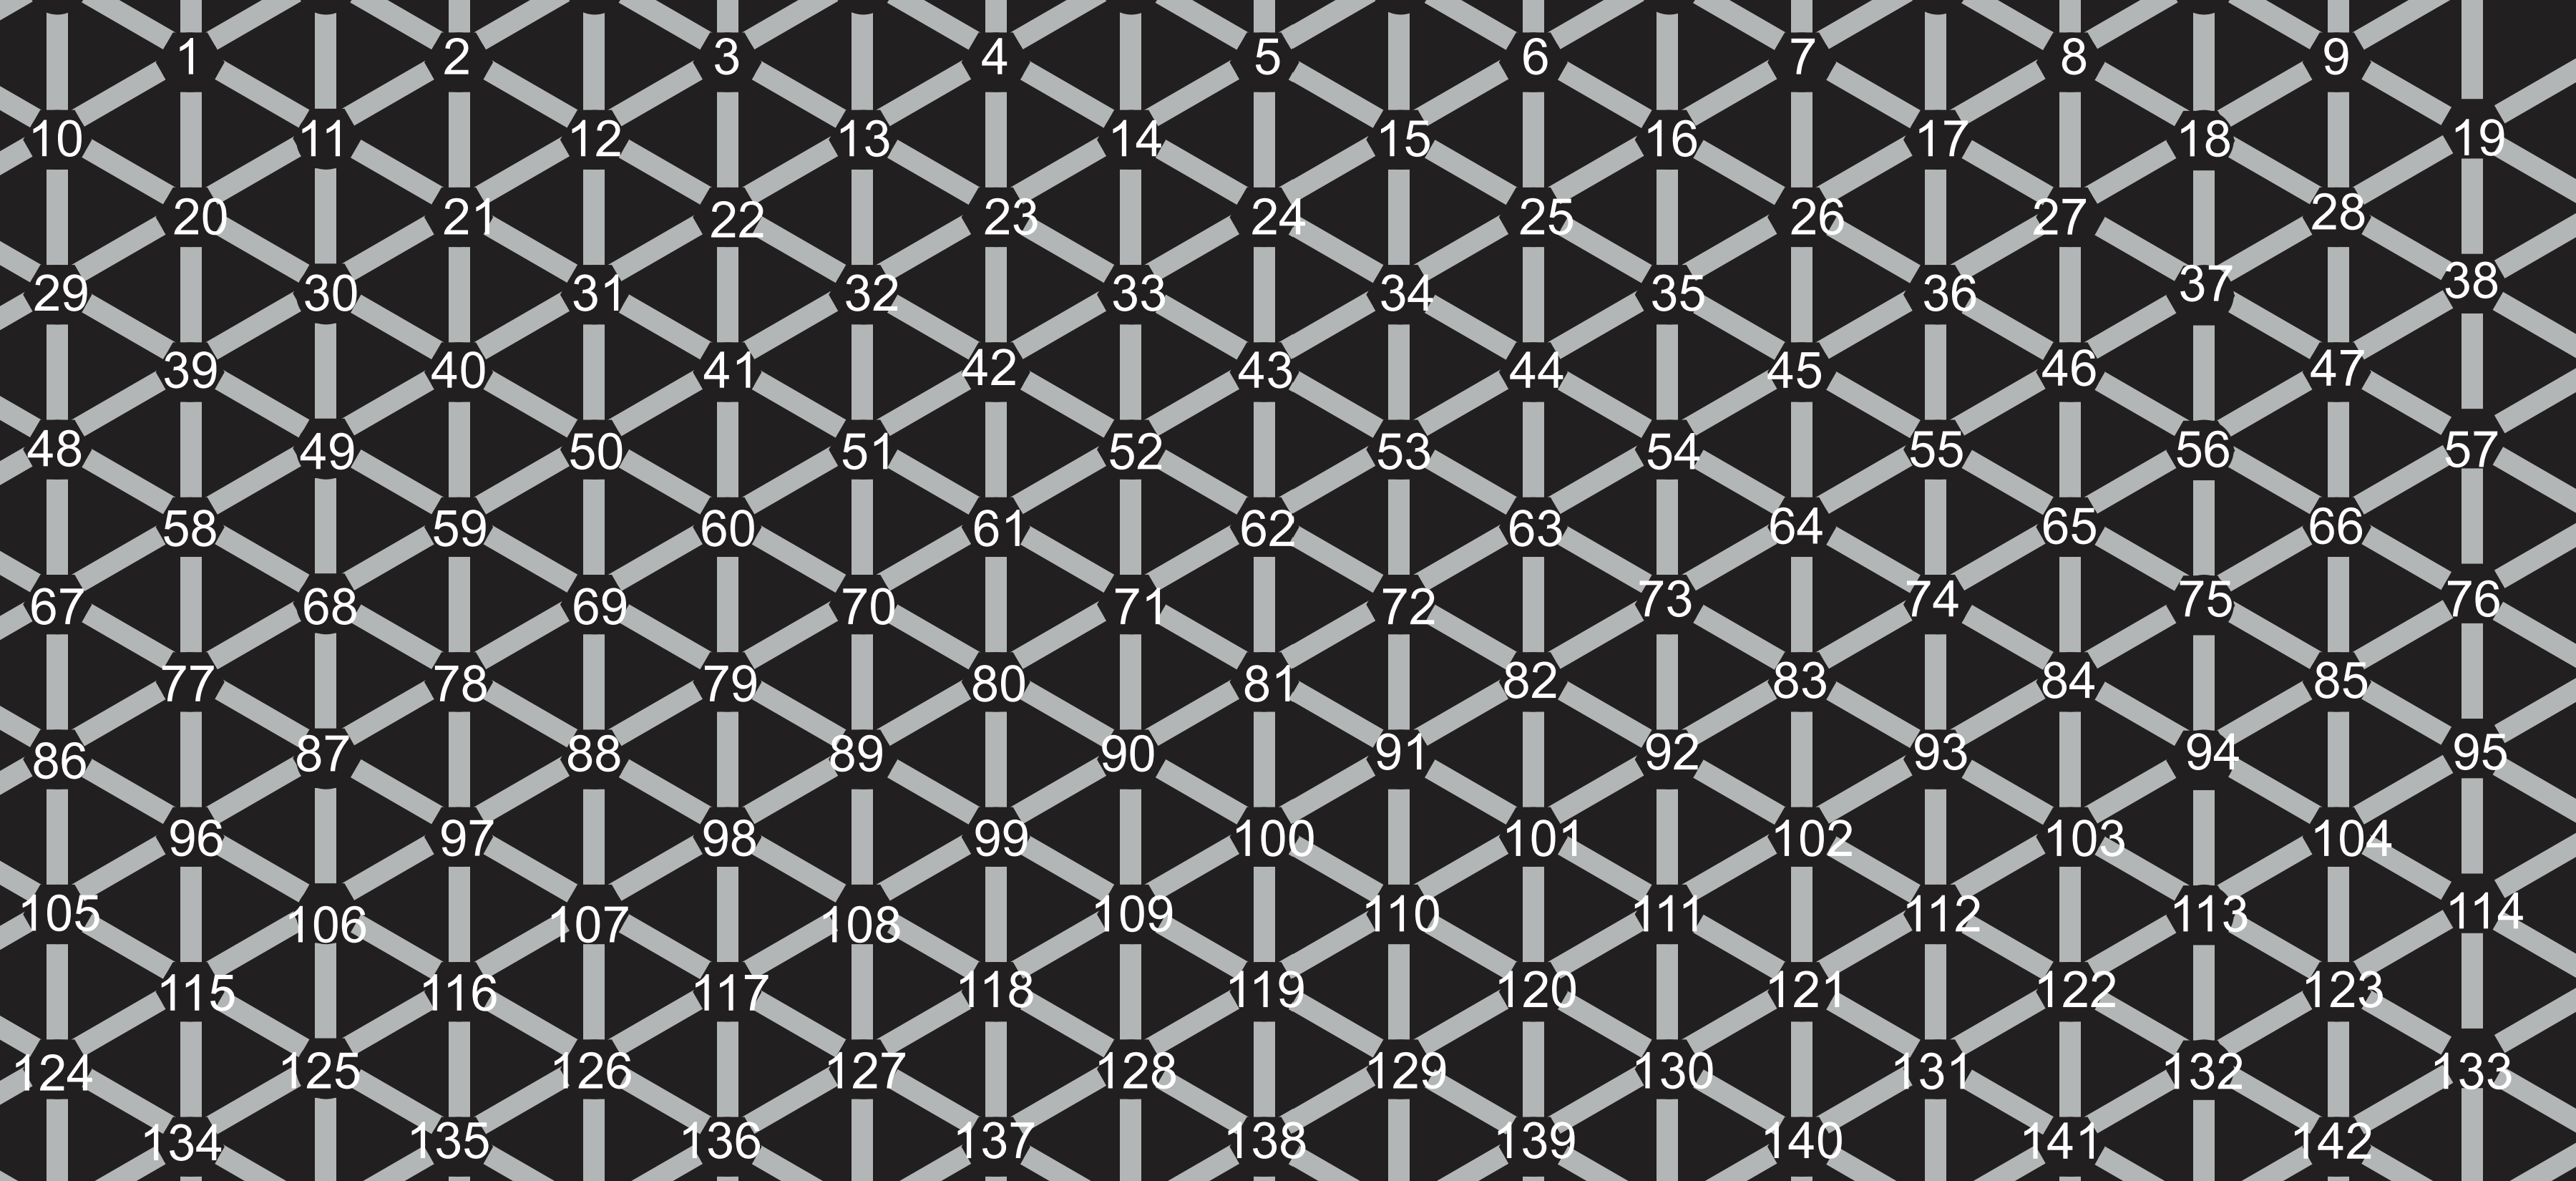
\includegraphics[scale = 0.3]{images/hexgrid_with_numbers.png}
    \caption{This shows the mat on the floor of the experimentation room which, upon which, the line following robots will navigate. The black and light grey lines can be detected by the line following robots' IR sensors.}
    \label{fig:hexgrid_with_numbers}
\end{figure}


% Section about the Khepera IV robot, their design and hence the limitations

The robots used in this maze are the \textit{Khepera IV} robots (see Fig. \ref{fig:robot}). On their bottom surface, they have IR sensors allowing them to detect when they have passed over a light grey line. 
This allows to them to keep track of the number of rotations they have made in place or the number of translations they have made. This allows reliable navigation the around the hexagonal space they inhabit.

Due to the parallel arrangement of the wheels on the underside of the robots, they are only able to move forwards and backwards or turn in place. In order to alter the direction of travel, the robots must first rotate \textit{and then} translate.

Therefore, whenever the platform robot wants to move to the out of its current direction of travel, it must first rotate to its desired direction of travel and then translate forwards.

\begin{figure}[h]
    \centering
    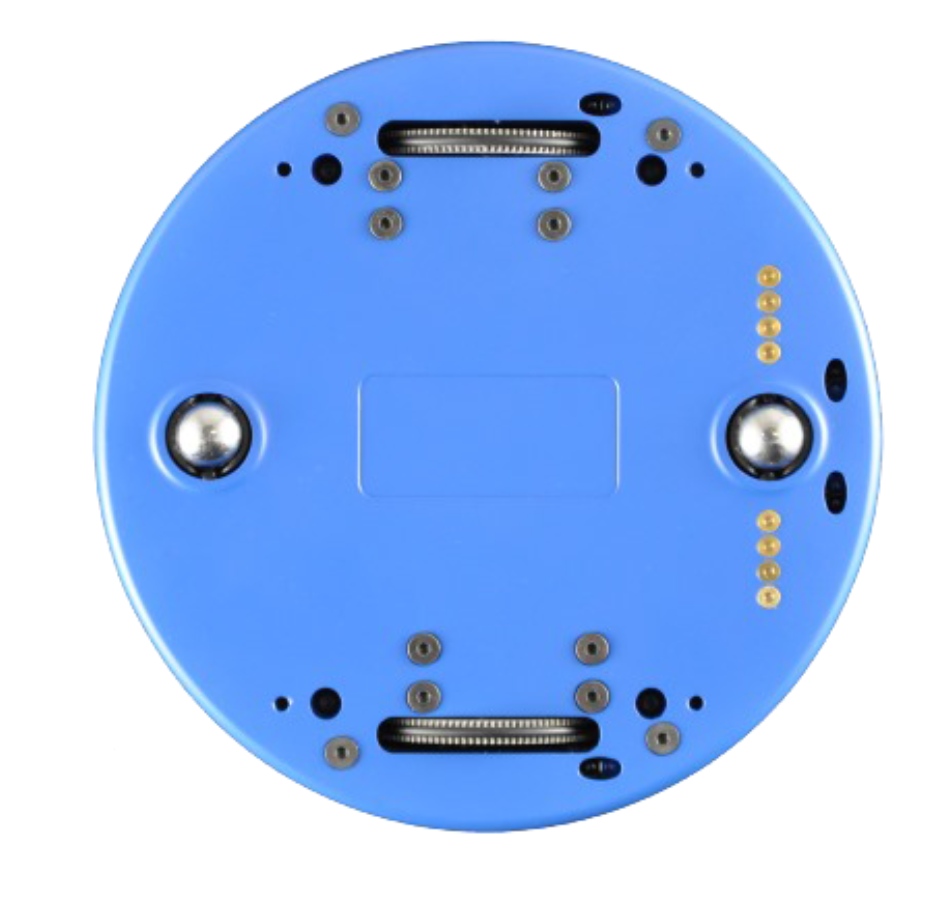
\includegraphics[scale = 0.5]{images/khepera_IV_robot.png}
    \caption{Shown is the underneath of the \textit{Khepera IV} robot. Note the presence of the 2 parralel wheels of the robot. This leads to signicant movement limitations of the \textit{Khepera IV} robots which must be addressed in the development of the program to control the Dynamic Honeycomb Maze.}
    \label{fig:robot}
\end{figure}

\subsection{Platforms}

%Section about the design of the platforms of the robot and the limitations that come with it
Due to the hexagonally tiled space, shown in Figure \ref{fig:collision}, consecutive tiles cannot rotate next to each other, otherwise they will collide.

\subsection{Summary of limitations of the line following robot and its platform.} 

Below are the intrinsic design constraints that the program will have to overcome for a successful Honeycomb Maze to be developed:
\begin{tcolorbox}
\begin{enumerate}
\item Two hexagonal platform \textit{that are adjacent} are unable to rotate without colliding. To avoid this, a robot cannot be adjacent to another robot when they rotate (see Fig \ref{fig:collision} for example collision).
\item Due to the parallel wheels of the robot, they have a sense of polarity, meaning they can not change direction without rotating first.
\end{enumerate}
\end{tcolorbox}
This results in a limited range of movement of the platforms when they are consecutive to each other and are in fact only able to move without restriction when they are not consecutive to any other platform robots.

\subsection{Development Environment}

%Justify the use of python 
The development of this package has been done in Python 3. This allows the integration of other libraries for simplifying the program.
The program developed, will return a list of commands that are given to the \textit{Khepera IV}. These will be executed by the  \textit{Khepera IV} to move around the hexagonal grid upon which it is placed.


% \subsection{Network of Integration}

% Explain how the python code will interact with the robots directly.

As the aim of this dissertation is to develop a tool for investigating the behaviour of mouse models, is it also an important aim for the program to be structured such a way that modifications to the code to add new behaviour in the future are possible


